\documentclass[10pt]{beamer}


\usepackage{xeCJK}
\setCJKmainfont{Noto Sans CJK SC}
\xeCJKsetup{PunctStyle=kaiming,CJKspace=true,CheckSingle=true} 

\usepackage{subfigure}
\usepackage{amssymb, amsmath, amsfonts,verbatim}
\usepackage{hyperref}
\usepackage{tikz}

\graphicspath{ {./} }
\usetikzlibrary{matrix,arrows,fit,backgrounds,mindmap,plotmarks,decorations.pathreplacing}
\usepackage{tkz-euclide}
\usetkzobj{all}
\usepackage{pgfplots}
\usepackage[xetex]{media9}
\pgfplotsset{compat=1.12}
\pgfdeclarelayer{background}
\pgfsetlayers{background,main}

\tikzset{decoration={name=none},}

\newlength\figureheight
\newlength\figurewidth

\newcommand{\tikzdir}[1]{#1.tikz}
\newcommand{\inputtikz}[1]{\input{\tikzdir{#1}}}

\newcommand{\tI}{\tilde {\mathcal I}}
\newcommand{\tA}{\tilde A}
\newcommand{\ty}{\tilde y}
\newcommand{\tx}{\tilde x}
\newcommand{\tw}{\tilde w}
\newcommand{\tv}{\tilde v}
\newcommand{\tC}{\tilde C}
\newcommand{\tP}{\tilde P}
\newcommand{\Ic}{{\mathcal I^c}}
\newcommand{\J}{{\mathcal J}}
\newcommand{\K}{{\mathcal K}}

\DeclareMathOperator{\Smin}{Smin}
\DeclareMathOperator{\Smid}{Smid}
\DeclareMathOperator{\Smax}{Smax}
\DeclareMathOperator{\MSE}{MSE}
\DeclareMathOperator{\rank}{rank}
\DeclareMathOperator{\Med}{Med}
\DeclareMathOperator{\Max}{Max}
\DeclareMathOperator{\Min}{Min}
\DeclareMathOperator{\tr}{tr}
\DeclareMathOperator{\Cov}{Cov}
\DeclareMathOperator{\logdet}{log\;det}
\DeclareMathOperator{\argmin}{arg\;min}
\DeclareMathOperator{\argmax}{arg\;max}
\let\Tiny\tiny

\title[Private Consensus]{分布式一致性问题中的隐私保护}
\author[Yilin Mo]{莫一林}
\institute[Tsinghua]{
  清华大学 自动化系
}
\date[Dec 5th, 2018]{Dec 5th, 2018}


\usetheme[subsectionpage=none,block=fill]{metropolis}
\definecolor{thupurple}{RGB}{102,8,116}
\definecolor{caltechcolor}{RGB}{102,8,116}
\setbeamercolor{title separator}{fg=black!50}
\setbeamercolor{frametitle}{bg=thupurple!70!black}


\begin{document}

\maketitle 
\section{An Illustrated Guide to a Ph.D.}

\begin{frame}{}
  Imagine a circle that contains all of human knowledge\footnote{By \href{http://matt.might.net/}{Matt Might}, \url{http://matt.might.net/articles/phd-school-in-pictures/}}:

  \begin{figure}[hb]
    \centering
    \includegraphics[width=0.8\textwidth]{images/PhDKnowledge-001.png}
  \end{figure}
\end{frame}


\begin{frame}{}
  By the time you finish elementary school, you know a little:
  \begin{figure}[hb]
    \centering
    \includegraphics[width=0.8\textwidth]{images/PhDKnowledge-002.png}
  \end{figure}
\end{frame}


\begin{frame}{}
  By the time you finish high school, you know a bit more:
  \begin{figure}[hb]
    \centering
    \includegraphics[width=0.8\textwidth]{images/PhDKnowledge-003.png}
  \end{figure}
\end{frame}


\begin{frame}{}
  With a bachelor's degree, you gain a specialty:
  \begin{figure}[hb]
    \centering
    \includegraphics[width=0.8\textwidth]{images/PhDKnowledge-004.png}
  \end{figure}
\end{frame}



\begin{frame}{}
  A master's degree deepens that specialty:
  \begin{figure}[hb]
    \centering
    \includegraphics[width=0.8\textwidth]{images/PhDKnowledge-005.png}
  \end{figure}
\end{frame}



\begin{frame}{}
  Reading research papers takes you to the edge of human knowledge:
  \begin{figure}[hb]
    \centering
    \includegraphics[width=0.8\textwidth]{images/PhDKnowledge-006.png}
  \end{figure}
\end{frame}


\begin{frame}{}
  Once you're at the boundary, you focus:
  \begin{figure}[hb]
    \centering
    \includegraphics[width=0.8\textwidth]{images/PhDKnowledge-007.png}
  \end{figure}
\end{frame}


\begin{frame}{}
  You push at the boundary for a few years:
  \begin{figure}[hb]
    \centering
    \includegraphics[width=0.8\textwidth]{images/PhDKnowledge-008.png}
  \end{figure}
\end{frame}

\begin{frame}{}
  Until one day, the boundary gives way:
  \begin{figure}[hb]
    \centering
    \includegraphics[width=0.8\textwidth]{images/PhDKnowledge-009.png}
  \end{figure}
\end{frame}


\begin{frame}{}
  And, that dent you've made is called a Ph.D.:

  \begin{figure}[hb]
    \centering
    \includegraphics[width=0.8\textwidth]{images/PhDKnowledge-010.png}
  \end{figure}
\end{frame}


\begin{frame}{}
  Of course, the world looks different to you now:
  \begin{figure}[hb]
    \centering
    \includegraphics[width=0.8\textwidth]{images/PhDKnowledge-011.png}
  \end{figure}
\end{frame}


\begin{frame}{}
  So, don't forget the bigger picture:
  \begin{figure}[hb]
    \centering
    \includegraphics[width=0.8\textwidth]{./images/PhDKnowledge-012.png}
  \end{figure}
\end{frame}

\begin{frame}{}
  \Huge Keep pushing.
\end{frame}

\section{分布式一致性算法}
\begin{frame}{集中式 v.s. 分布式算法}
  \begin{figure}[<+htpb+>]
    \begin{center}
      \includegraphics[width=0.50\textwidth]{centralized.png}
    \end{center}
  \end{figure}
  分布式算法的好处:可靠、可扩展
\end{frame}

\begin{frame}{分布式平均一致性算法}
  \begin{center}
    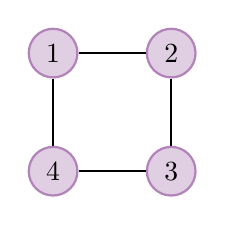
\begin{tikzpicture}
      \node (n4) at (0,0) [circle,draw=thupurple!50,fill=thupurple!20,thick] {4};
      \node (n1) at (0,1.5cm) [circle,draw=thupurple!50,fill=thupurple!20,thick] {1};
      \node (n3) at (1.5cm,0) [circle,draw=thupurple!50,fill=thupurple!20,thick] {3};
      \node (n2) at (1.5cm,1.5cm) [circle,draw=thupurple!50,fill=thupurple!20,thick] {2};
      \draw [semithick] (n1)--(n2)--(n3)--(n4)--(n1);
    \end{tikzpicture}
  \end{center}
  \begin{itemize}
  \item 4个节点,每个节点具有初始值$x_i(0)$。
  \item 目标: 计算初始值的平均值。
  \item 每次迭代,各节点使用如下的方程更新自身状态:
    \begin{align*}
      x_i(k+1) =  \frac{1}{3}x_{i}(k) + \sum_{j\in \mathcal N(i)} \frac{1}{3} x_{j}(k).  
    \end{align*}
  \end{itemize}
\end{frame}

\begin{frame}{状态轨迹}
  \begin{figure}[ht]
    \centering
    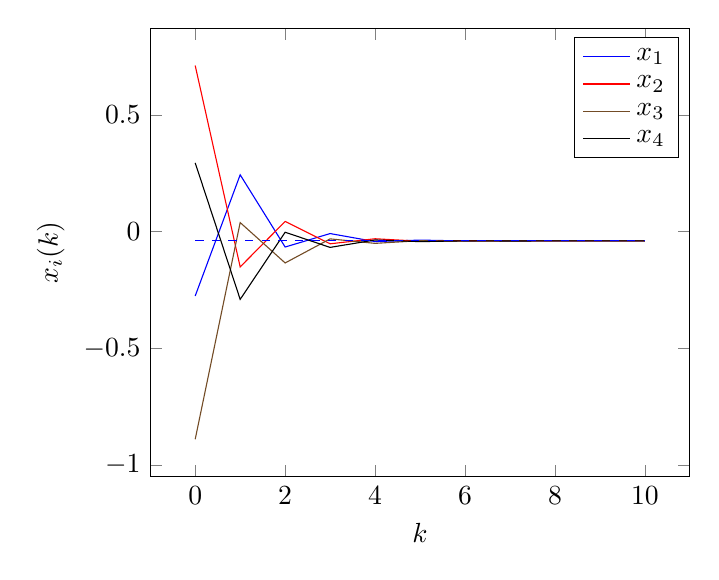
\begin{tikzpicture}[]
  \begin{axis}[ylabel = {$x_i(k)$}, xlabel = {$k$}]\addplot+ [mark = {none}]coordinates {
      (0.0, -0.2755239333343977)
      (1.0, 0.24342693842600588)
      (2.0, -0.06595015324993514)
      (3.0, -0.008288945276556974)
      (4.0, -0.04266417768499486)
      (5.0, -0.03625737679906395)
      (6.0, -0.040076847066668156)
      (7.0, -0.03936498030156472)
      (8.0, -0.039789365886854076)
      (9.0, -0.03971026957962036)
      (10.0, -0.03975742353354139)
    };
    \addlegendentry{$x_1$}
    \addplot+ [mark = {none}]coordinates {
      (0.0, 0.711289173226358)
      (1.0, -0.15117643278118886)
      (2.0, 0.043695747479037705)
      (3.0, -0.05213376429957861)
      (4.0, -0.0304812998262201)
      (5.0, -0.04112902335717746)
      (6.0, -0.03872319397124874)
      (7.0, -0.03990627436357733)
      (8.0, -0.039638959987363026)
      (9.0, -0.03977041336428842)
      (10.0, -0.03974071176693128)
    };
    \addlegendentry{$x_2$}
    \addplot+ [mark = {none}]coordinates {
      (0.0, -0.889294538235527)
      (1.0, 0.0388367367922961)
      (2.0, -0.1341468871278384)
      (3.0, -0.031021189902524723)
      (4.0, -0.05024159256031744)
      (5.0, -0.03878318175750481)
      (6.0, -0.040918782052815114)
      (7.0, -0.03964562529694704)
      (8.0, -0.03988291421864818)
      (9.0, -0.03974145235688506)
      (10.0, -0.039767817792629626)
    };
    \addlegendentry{$x_3$}
    \addplot+ [mark = {none}]coordinates {
      (0.0, 0.2945155753860573)
      (1.0, -0.29010096539462243)
      (2.0, -0.002612430058773485)
      (3.0, -0.067569823478849)
      (4.0, -0.0356266528859769)
      (5.0, -0.042844141043763065)
      (6.0, -0.03929489986677727)
      (7.0, -0.04009684299542018)
      (8.0, -0.03970248286464398)
      (9.0, -0.03979158765671541)
      (10.0, -0.03974776986440694)
    };
    \addlegendentry{$x_4$}
    \addplot+ [mark = {none}, dashed]coordinates {
      (0.0, -0.03975343073937733)
      (10.0, -0.03975343073937733)
    };
  \end{axis}

\end{tikzpicture}
  \end{figure}
\end{frame}

\begin{frame}{分布式平均一致性理论}
  \begin{itemize}
  \item 假设系统的拓扑可以由$G = \{V,\,E\}$表示。
  \item 节点更新方程:
    \begin{displaymath}
      x_i(k+1) = a_{ii} x_{i}(k) + \sum_{j\in \mathcal N(i)} a_{ij} x_{j}(k).  
    \end{displaymath}
  \item 矩阵表示:
    \begin{displaymath}
      x(k+1) = A x(k),
    \end{displaymath}
  \item 以下条件为达成平均一致性的充要条件:
    \begin{enumerate}
    \item[(A1)] $A$有一个特征值是$1$,其他所有特征值在单位圆内。 
    \item[(A2)] $\mathbf 1$是对应特征值$1$的左特征向量和右特征向量。
    \end{enumerate}
  \end{itemize}
\end{frame}


\begin{frame}{平均一致性的应用}
  \begin{itemize}
  \item 需求相应;
  \item 多机器人队型控制;
  \item 社交网络;
  \item 时钟同步;
  \item 分布式定位;
  \item 分布式估计;
  \item 分布式优化;
  \item \dots
  \end{itemize}
\end{frame}

\section{分布式算法中的安全问题}
\begin{frame}{安全隐患}
  \begin{itemize}
  \item 恶意节点:不遵守更新方程 
    \begin{displaymath}
      x_i(k+1) = a_{ii} x_{i}(k) + \sum_{j\in \mathcal N(i)} a_{ij} x_{j}(k)+\textcolor{red}{u_i(k)}.
    \end{displaymath}

    \emph{(Pasqualetti, Bicchi and Bullo, 2012)}: 当图$G$足够联通时,好的节点可以辨识出恶意节点

  \item 好奇节点:遵守更新方程,但是尝试推测其他节点的状态
  \item 恶意+好奇节点:Open Problem 
  \end{itemize}
\end{frame}

\begin{frame}{Example}
  \begin{center}
    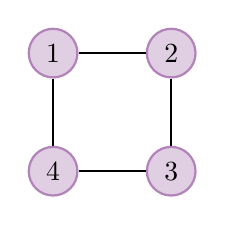
\begin{tikzpicture}
      \node (n4) at (0,0) [circle,draw=thupurple!50,fill=thupurple!20,thick] {4};
      \node (n1) at (0,1.5cm) [circle,draw=thupurple!50,fill=thupurple!20,thick] {1};
      \node (n3) at (1.5cm,0) [circle,draw=thupurple!50,fill=thupurple!20,thick] {3};
      \node (n2) at (1.5cm,1.5cm) [circle,draw=thupurple!50,fill=thupurple!20,thick] {2};
      \draw [semithick] (n1)--(n2)--(n3)--(n4)--(n1);
    \end{tikzpicture}
  \end{center}
  \begin{itemize}
  \item 第一次迭代:节点$4$可以得到$x_1(0)$以及$x_3(0)$.
  \item 第二次迭代:节点$4$可以得到$x_1(1)$:
    \begin{align*}
      x_1(1) =\frac{1}{3}\left(\underbrace{x_1(0)+x_4(0)}_{known}+x_2(0)\right).
    \end{align*}
  \item 对于一般系统,判断节点$i$能否准确推测节点$j$的初始值,涉及到线性系统的可观性理论
  \end{itemize}
\end{frame}

\begin{frame}{方案1}
  \begin{figure}[ht]
    \begin{center}
      \begin{tikzpicture}[scale=0.9]
        \node [label=above:$k:$] at (-1.5,0) {};
        \node [label=above:$0$] at (0,0) {};
        \node [label=above:$1$] at (3,0) {};
        \node [label=above:$2$] at (6,0) {};
        \node [label=above:$3$] at (9,0) {};
        \node []   at (-1.5,-1) {噪声:};
        \node [] (n0) at (0,-1){$v_i(0)$}; 
        \node [] (n1) at (3,-1){$ v_i(1)$}; 
        \node [] (n2) at (6,-1){$ v_i(2)$}; 
        \node [] (n3) at (9,-1){$ v_i(3)$}; 
        \draw [->,thick] (n0)--(n1);
        \draw [->,thick] (n1)--(n2);
        \draw [->,thick] (n2)--(n3);
      \end{tikzpicture}
    \end{center}
  \end{figure}
\end{frame}
\begin{frame}{状态轨迹}
  \begin{figure}[ht]
    \centering
    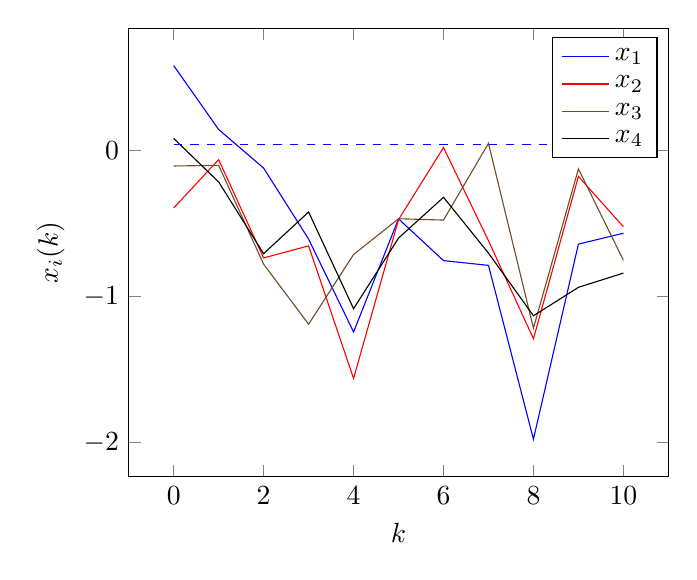
\begin{tikzpicture}[]
  \begin{axis}[ylabel = {$x_i(k)$}, xlabel = {$k$}]\addplot+ [mark = {none}]coordinates {
      (0.0, 0.5830254744902436)
      (1.0, 0.14476988310455036)
      (2.0, -0.11941848097706835)
      (3.0, -0.6059757863739825)
      (4.0, -1.2430834369626589)
      (5.0, -0.46756232010277327)
      (6.0, -0.7537704571731478)
      (7.0, -0.7864188425513643)
      (8.0, -1.9776832284946848)
      (9.0, -0.6407132184127148)
      (10.0, -0.5660666929387985)
    };
    \addlegendentry{$x_1$}
    \addplot+ [mark = {none}]coordinates {
      (0.0, -0.392992596435168)
      (1.0, -0.06158705533014694)
      (2.0, -0.7355018497199227)
      (3.0, -0.6526852673027316)
      (4.0, -1.5611711199300813)
      (5.0, -0.4725902764469253)
      (6.0, 0.021511578999348108)
      (7.0, -0.6174717034105712)
      (8.0, -1.289406915104661)
      (9.0, -0.17657142664220865)
      (10.0, -0.521900592415504)
    };
    \addlegendentry{$x_2$}
    \addplot+ [mark = {none}]coordinates {
      (0.0, -0.10512990958943226)
      (1.0, -0.1010331714343752)
      (2.0, -0.7786017907371763)
      (3.0, -1.1894802974422716)
      (4.0, -0.711800310578502)
      (5.0, -0.46682762733025807)
      (6.0, -0.47577425735040935)
      (7.0, 0.04990830814323197)
      (8.0, -1.2166014426746194)
      (9.0, -0.12479825345136457)
      (10.0, -0.7515139797672027)
    };
    \addlegendentry{$x_3$}
    \addplot+ [mark = {none}]coordinates {
      (0.0, 0.08355798272700599)
      (1.0, -0.21443808082314028)
      (2.0, -0.7061710238939025)
      (3.0, -0.4203765163363313)
      (4.0, -1.083368574769455)
      (5.0, -0.5991671093029338)
      (6.0, -0.319770078708885)
      (7.0, -0.7021793494992539)
      (8.0, -1.1317305740180243)
      (9.0, -0.9369523823018764)
      (10.0, -0.8392146846434922)
    };
    \addlegendentry{$x_4$}
    \addplot+ [mark = {none}, dashed]coordinates {
      (0.0, 0.04211523779816233)
      (10.0, 0.04211523779816233)
    };
  \end{axis}

\end{tikzpicture}

  \end{figure}
\end{frame}


\begin{frame}{方案2}
  \begin{figure}[ht]
    \begin{center}
      \begin{tikzpicture}[scale=0.9]
        \node [label=above:$k:$] at (-1.5,0) {};
        \node [label=above:$0$] at (0,0) {};
        \node [label=above:$1$] at (3,0) {};
        \node [label=above:$2$] at (6,0) {};
        \node [label=above:$3$] at (9,0) {};
        \node [] at (-1.5,-1) {噪声:};
        \node [] (n0) at (0,-1){$v_i(0)$}; 
        \node [] (n1) at (3,-1){$\varphi v_i(1)$}; 
        \node [] (n2) at (6,-1){$\varphi^2 v_i(2)$}; 
        \node [] (n3) at (9,-1){$\varphi^3 v_i(3)$}; 
        \draw [->,thick] (n0)--(n1);
        \draw [->,thick] (n1)--(n2);
        \draw [->,thick] (n2)--(n3);
      \end{tikzpicture}
    \end{center}
  \end{figure}
\end{frame}
\begin{frame}{状态轨迹}
  \begin{figure}[ht]
    \centering
    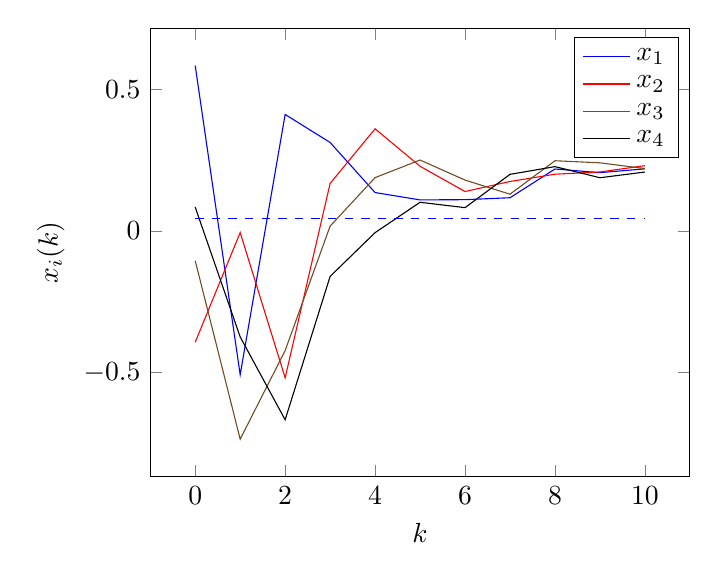
\begin{tikzpicture}[]
  \begin{axis}[ylabel = {$x_i(k)$}, xlabel = {$k$}]\addplot+ [mark = {none}]coordinates {
      (0.0, 0.5830254744902436)
      (1.0, -0.5073856496340193)
      (2.0, 0.4105926826053661)
      (3.0, 0.31178041883330665)
      (4.0, 0.13511616469793258)
      (5.0, 0.109173046680069)
      (6.0, 0.1100506367509752)
      (7.0, 0.11684064159139178)
      (8.0, 0.2182232606358762)
      (9.0, 0.20530712266919754)
      (10.0, 0.21875296490192422)
    };
    \addlegendentry{$x_1$}
    \addplot+ [mark = {none}]coordinates {
      (0.0, -0.392992596435168)
      (1.0, -0.006049626240259232)
      (2.0, -0.5183864801127663)
      (3.0, 0.16727923587002402)
      (4.0, 0.3599419605508179)
      (5.0, 0.22783454943465606)
      (6.0, 0.13870045665343825)
      (7.0, 0.1741551692913772)
      (8.0, 0.19981205402232516)
      (9.0, 0.20780088492798154)
      (10.0, 0.2299610353221999)
    };
    \addlegendentry{$x_2$}
    \addplot+ [mark = {none}]coordinates {
      (0.0, -0.10512990958943226)
      (1.0, -0.7348928814915329)
      (2.0, -0.42224553595848935)
      (3.0, 0.016699464194805003)
      (4.0, 0.18776277952977122)
      (5.0, 0.2498755515435507)
      (6.0, 0.17910797331149172)
      (7.0, 0.1292873106365846)
      (8.0, 0.24734826369352908)
      (9.0, 0.23997245548825497)
      (10.0, 0.21970652819232567)
    };
    \addlegendentry{$x_3$}
    \addplot+ [mark = {none}]coordinates {
      (0.0, 0.08355798272700599)
      (1.0, -0.3741819536538027)
      (2.0, -0.6664072691055933)
      (3.0, -0.16075290183402352)
      (4.0, -0.0062699875819918205)
      (5.0, 0.1007978967426149)
      (6.0, 0.08183599669764424)
      (7.0, 0.1993378268436817)
      (8.0, 0.22655506324603128)
      (9.0, 0.1873758996180442)
      (10.0, 0.2075457558531128)
    };
    \addlegendentry{$x_4$}
    \addplot+ [mark = {none}, dashed]coordinates {
      (0.0, 0.04211523779816233)
      (10.0, 0.04211523779816233)
    };
  \end{axis}

\end{tikzpicture}
  \end{figure}
\end{frame}


\begin{frame}{方案3}
  \begin{figure}[ht]
    \begin{center}
      \begin{tikzpicture}[scale=0.9]
        \node [label=above:$k:$] at (-1.5,0) {};
        \node [label=above:$0$] at (0,0) {};
        \node [label=above:$1$] at (3,0) {};
        \node [label=above:$2$] at (6,0) {};
        \node [label=above:$3$] at (9,0) {};
        \node []   at (-1.5,-1) {噪声:};
        \node [] (n0) at (0,-1){$v_i(0)$}; 
        \node [] (n1) at (3,-1){$\begin{array}{c}\textcolor{red}{\varphi v_i(1)}\\+\\- v_i(0)\end{array}$}; 
        \node [] (n2) at (6,-1){$\begin{array}{c}\textcolor{blue}{\varphi^2 v_i(2)}\\+\\\textcolor{red}{- \varphi v_i(1)}\end{array}$}; 
        \node [] (n3) at (9,-1){$\begin{array}{c}\textcolor{thupurple}{\varphi^3 v_i(3)}\\+\\\textcolor{blue}{ -\varphi^2 v_i(2)}\end{array}$}; 
        \draw [->,thick] (n0)--(n1);
        \draw [->,thick] (n1)--(n2);
        \draw [->,thick] (n2)--(n3);
      \end{tikzpicture}
    \end{center}
  \end{figure}
\end{frame}
\begin{frame}{状态轨迹}
  \begin{figure}[ht]
    \centering
    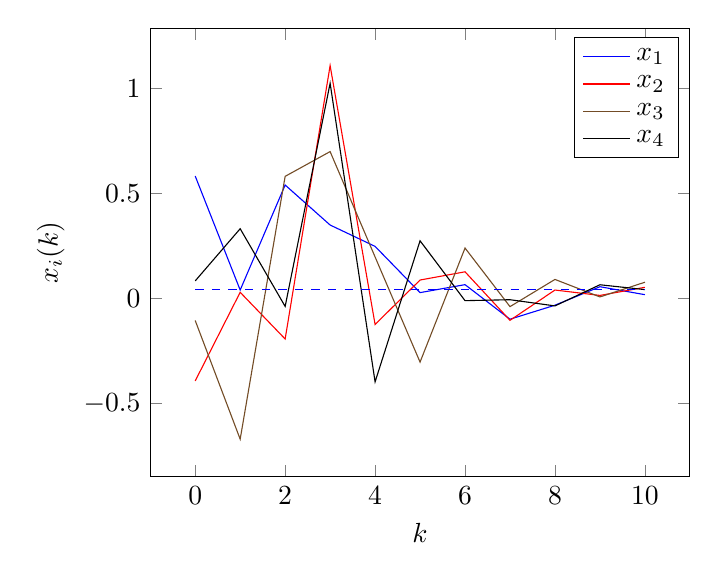
\begin{tikzpicture}[]
  \begin{axis}[ylabel = {$x_i(k)$}, xlabel = {$k$}]\addplot+ [mark = {none}]coordinates {
      (0.0, 0.5830254744902436)
      (1.0, 0.040149182564258104)
      (2.0, 0.5403713847075715)
      (3.0, 0.3498323383157756)
      (4.0, 0.24806006746048426)
      (5.0, 0.0277678671652557)
      (6.0, 0.06571483976768719)
      (7.0, -0.09890491838031368)
      (8.0, -0.032224656543781705)
      (9.0, 0.05583294953987378)
      (10.0, 0.017949407150518827)
    };
    \addlegendentry{$x_1$}
    \addplot+ [mark = {none}]coordinates {
      (0.0, -0.392992596435168)
      (1.0, 0.029295199206055885)
      (2.0, -0.19318318304261484)
      (3.0, 1.1094561200369628)
      (4.0, -0.12403930298855464)
      (5.0, 0.08774876084095368)
      (6.0, 0.126922177399341)
      (7.0, -0.10422740989324977)
      (8.0, 0.04007471887738956)
      (9.0, 0.014362096070200912)
      (10.0, 0.05307920466232918)
    };
    \addlegendentry{$x_2$}
    \addplot+ [mark = {none}]coordinates {
      (0.0, -0.10512990958943226)
      (1.0, -0.6705215555225883)
      (2.0, 0.5817149090286323)
      (3.0, 0.699707160970051)
      (4.0, 0.1976779771894504)
      (5.0, -0.3033529340182755)
      (6.0, 0.24013151712015665)
      (7.0, -0.03898963282873712)
      (8.0, 0.09062333259240149)
      (9.0, 0.0072551335621690305)
      (10.0, 0.07729872847186198)
    };
    \addlegendentry{$x_3$}
    \addplot+ [mark = {none}]coordinates {
      (0.0, 0.08355798272700599)
      (1.0, 0.3322152151142626)
      (2.0, -0.03804604888061086)
      (3.0, 1.0253167102007776)
      (4.0, -0.39752407354514563)
      (5.0, 0.27485061026356467)
      (6.0, -0.010537386830266438)
      (7.0, -0.006066342697308512)
      (8.0, -0.03555591161152922)
      (9.0, 0.06514113372466127)
      (10.0, 0.042125352833851396)
    };
    \addlegendentry{$x_4$}
    \addplot+ [mark = {none}, dashed]coordinates {
      (0.0, 0.04211523779816233)
      (10.0, 0.04211523779816233)
    };
  \end{axis}

\end{tikzpicture}

  \end{figure}
\end{frame}

\begin{frame}{隐私保护}
  \begin{figure}[ht]
    \begin{center}
      \setlength{\figureheight}{5cm}
      \setlength{\figurewidth}{6cm}
      \inputtikz{variance}
    \end{center}
    \label{fig:variance}
  \end{figure}
\end{frame}

\section{控制系统中的信息安全问题}
\begin{frame}{震网病毒}
  \begin{figure}[ht]
    \centering
    \includegraphics[width=0.8\textwidth]{stuxnet.jpg}
  \end{figure}
  震网病毒于2010年6月被发现,它是第一个可以对控制系统产生破坏的恶意软件。
\end{frame}

\begin{frame}{工业控制系统中的安全隐患}
  \begin{figure}[ht]
    \centering
    \includegraphics[width=0.6\textwidth]{cert.jpg}
  \end{figure}
  2014年,美国工业控制系统应急小组收到245起针对工业控制系统的攻击报告。2016年,攻击数量增加至290起。
\end{frame}

\begin{frame}[standout]
  感谢各位老师同学聆听,请大家批评指正!
\end{frame}
\begin{frame}
  \includemedia[width=0.6\linewidth,height=0.6\linewidth,activate=pageopen,
  passcontext,
  transparent,
  addresource=penguinschasingbutterfly.mp4,
  flashvars={source=penguinschasingbutterfly.mp4}
  ]{\includegraphics[width=0.6\linewidth]{penguins}}{VPlayer.swf}
\end{frame}
\end{document}

%%% Local Variables: 
%%% coding: utf-8
%%% mode: latex
%%% TeX-engine: xetex
%%% End: 